\documentclass[12pt]{report}
\usepackage{braket}
\usepackage{physics}
\usepackage{graphicx}
\usepackage{times}
\usepackage[export]{adjustbox}
\usepackage{listings}
\usepackage{mathcomp}
% \usepackage{hyperref}
\usepackage{bm,amsmath}
\usepackage{float}
\usepackage{indentfirst}
\usepackage{bigints}
\usepackage{listings}
\usepackage{color}

\usepackage[xindy, splitindex]{imakeidx}
\makeindex[
	columns=2,
	program=truexindy,
	intoc=true,
	options=-M texindy -I xelatex -C utf8,
	title={index}
    ]
\usepackage[unicode, bookmarksnumbered]{hyperref}
\definecolor{dkgreen}{rgb}{0,0.6,0}
\definecolor{gray}{rgb}{0.5,0.5,0.5}
\definecolor{mauve}{rgb}{0.58,0,0.82}

\lstset{frame=tb,
  language=Python,
  aboveskip=3mm,
  belowskip=3mm,
  stepnumber = 1,
  showstringspaces=false,
  columns=flexible,
  basicstyle={\small\ttfamily},
  numbers=left,
  numberstyle=\color{gray},
  keywordstyle=\color{blue},
  commentstyle=\color{dkgreen},
  stringstyle=\color{mauve},
  breaklines=true,
  breakatwhitespace=true,
  tabsize=3
}

\numberwithin{equation}{section}

\title{Application of Particle Net}
\author{Ting-Kai Hsu}
\date{}

\begin{document}
\maketitle
\tableofcontents

\chapter{ParticleNet Structure}
\section{Notification}
Note that the requirement for running Particle Net is important.
One thing to note that the version of \textbf{numpy} should below 1.14.1, and professor suggestes to run the program on Linux system.

\section{stack\_arrays}
First, it has defined two functions dealing with the data format, 

\begin{itemize}
    \item stack\_arrays
    \item pad\_arrays
\end{itemize}

For the first function, the definition code would be,
\begin{lstlisting}
def stack_arrays(a, keys, axis=-1):
    flat_arr = np.stack([a[k].flatten() for k in keys], axis=axis)
    return awkward.JaggedArray.fromcounts(a[keys[0]].counts, flat_arr)
\end{lstlisting}

For the first, we have to know what is \textbf{np.stack()}, it is a function that can reconstruct some arrays and then combine (stack) them. The parameter \textbf{axis} would be the orientation of the seperation.
In this case, \textbf{axis = -1}, which means the array would construct along their last axis, like below.
\begin{figure}[H]
    \centering
    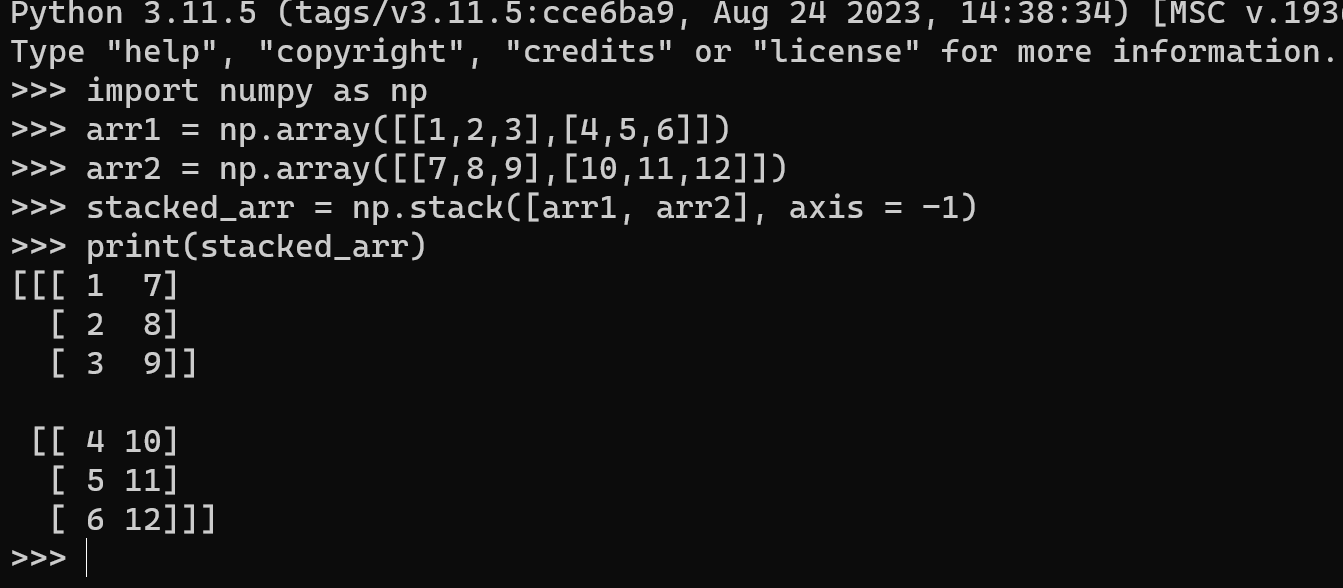
\includegraphics[width=\linewidth]{np.stack.png}
    \caption{Example for np.stack([ , ], axis = -1)}
    \label{1}
\end{figure}

Also, the function \textbf{flatten()} would flatten the array into 1 dimesion array.
Let's move on to the line 3, where we use the package \textbf{awkward}.

\begin{itemize}
    \item \textbf{a[keys[0]].counts}: this is the first argument of the function call. It would define the structure of the jagged array. Counts function would specify the number of elements in the suggested array.
    \item \textbf{flat\_arr}: this is the stack array created in line 2, and this argument would provide the data for the jagged array.
\end{itemize}

For example, if \textbf{a[keys[0]].counts} is [3, 2, 4], it means the JaggedArray will consist of three sublists, each with a different number of elements: 3, 2, and 4. 
The data in \textbf{flat\_arr} will be distributed into these sublists based on this structure.
\\
\indent This is a common operation when working with structured data, such as particle physics data, where events may have varying numbers of particles, and you need to represent the data in a structured, variable-length format.

\section{pad\_arrays}

\begin{lstlisting}
def pad_array(a, maxlen, value=0., dtype='float32'):
    x = (np.ones((len(a), maxlen)) * value).astype(dtype)
    for idx, s in enumerate(a):
        if not len(s):
            continue
        trunc = s[:maxlen].astype(dtype)
        x[idx, :len(trunc)] = trunc
    return x
\end{lstlisting}

First of all, we should explain what is the term 'padding' means. 
Padding is a common operation that we adjust the length of sequences to make them uniform. 
In our code, we use this function that takes a list of sequences to pad them with a maximum limitation to ensure them to have same length. 
Padding is a preprocess that do the data to the ML model which requires the inputs to have same dimensions.
Here we explain the code line by line,
For inputs, we have
\begin{itemize}
    \item \textbf{a}: The datatype would be array, which would provide the data that we should process.
    \item \textbf{maxlen}: The datatype would be integer, which would limit the length of the padded array.
    \item \textbf{value=0}: The datatype would be integer, and it would determine the initial content of padding with default value 0.
    \item \textbf{dtype='float32'}: This would determine the datatype stored in the array.
\end{itemize} 

Next we initialize the padded array,
\begin{lstlisting}
x = (np.ones((len(a), maxlen)) * value).astype(dtype)
\end{lstlisting}

We create a Numpy array \textbf{x} with dimension \textbf{(len(a), maxlen)} and then fill it with all zero. 
Note that the elements become zeros because the default value of \textbf{value} is zero, and \textbf{np.ones()} provides us flexibility to adjust the content of the array rather than making them all zero by \textbf{np.zeros()}.
Then we make the datatype of the elements become float32.
Next, let's move on to the for loop.
In the for loop, we go through the input list of sequences \textbf{a}, and \textbf{idx} would be the index of sequence, and \textbf{s} would be the sequence itself. First, we would check whether the sequence \textbf{s} is empty or not. If is empty, then the loop would skip and go on to the next loop. If is not empty, then we see line 6 and 7 together.

\begin{lstlisting}
    trunc = s[:maxlen].astype(dtype)
    x[idx, :len(trunc)] = trunc
\end{lstlisting}

First \textbf{trunc} means that we only take part of information of \textbf{s}, that is, we truncate the sequence for a certain length \textbf{maxlen}. For sequences that are shorter than \textbf{maxlen}, we pad the remaining part in \textbf{x} by \textbf{value}.

\section{Dataset--\_\_init\_\_()}

Dataset has been seperated into many parts, first we would introduce a function called \textbf{\_\_init\_\_}.

\begin{lstlisting}
def __init__(self, filepath, feature_dict = {}, label='label', pad_len=100, dataformat='channel_first'):
    self.filepath = filepath
    self.feature_dict = feature_dict
    if len(feature_dict)==0:
        feature_dict['points'] = ['part_etarel', 'part_phirel']
        feature_dict['feature'] = ['part_pt_log', 'part_e_log', 'part_etarel', 'part_phirel']
        feature_dict['mask'] = ['part_pt_log']
    self.label = label
    self.pad_len = pad_len
    assert data_format in ('channel_first', 'channel_last')
    self.stack_axis = 1 if data_format=='channel_first' else -1
    self._values = {}
    self._label = None
    self._load()
\end{lstlisting}

This function is obviously initialize the object with some certain inputs. \\
\textit{\textbf{Inputs}}: 
\begin{itemize}
    \item \textbf{self}: This is the parameter calling the object itself.
    \item \textbf{filepath}: This is the parameter that the data file comes from. 
    It is associated with the instance variable \textbf{self.filepath} which store the path of the data file.
    \item \textbf{self.feature\_dict = feature\_dict}: This variable is used to store a dictionary\footnote{Dictionary in Python is like map in C++, where there is key one-one to the data, and we can use the key to find the desired data.} of features. 
\end{itemize}

And then we go into a loop that initializes \textbf{feature\_dict}. First, we have to check whether the dictionary is empty or not, if not, we must advoid to overwrite the content; if so, we would do some works as shown below,
\begin{itemize}
    \item \textbf{feature\_dict['points'] = ['part\_etarel', 'part\_phirel']}: We assign a list of strings to a key \textbf{'points'}, and this may be the information (coordinates) of the particle with angular information.
    \item \textbf{feature\_dict['feature'] = ['part\_pt\_log', 'part\_e\_log', 'part\_etarel', 'part\_phirel']}:
    We assign the key \textbf{feature} to the some physical features\footnote{I don't know why but we neglect the information of charge carried by the particle here.} of the particle. In this case, we only provide some basic data, that is, the transverse momentum of the particle along the detector axis, energy of the particle, and the position of the particle we have mentioned previously. 
    \item \textbf{feature\_dict['mask'] = ['part\_pt\_log']}: \underline{This needs verification.}
    \item \textbf{stack\_axis}: This would tell us how transform the initial data format (may be channels\_first) to \hyperref[sec::channel]{channels\_last} by applying numpy.stack().\underline{How does this affect to the data would need discussion.} 
\end{itemize}

Next we need to review the meaning and function of \textbf{assert}. \textbf{assert} function is used to check at some certain time, what is the situation of the system. 
If the situation of assertion is different with the situation of the systen, the computer would print out the error message. \footnote{Check \hyperlink{https://openhome.cc/zh-tw/python/exception/assert/}{this}} 
So line 10 check whehter \textbf{dataformat} is in \textbf{'channel\_first'} or \textbf{'channel\_last}.
\\
\indent At the last line of this function, that is, line 14, the function calls another function called \textbf{\_load()}, which we would explain next.

\section{Dataset--\_load()}

After initializing the dataclass object, we now go through the function that reads the data file.

\begin{lstlisting}
def _load(self):
    logging.info('Start loading file %s' % self.filepath)
    counts = None
    with awkward.load(self.filepath) as a:
        self._label = a[self.label]
        for k in self.feature_dict:
            cols = self.feature_dict[k]
            if not isinstance(cols, (list, tuple)):
            cols = [cols]
            arrs = []
            for col in cols:
                if counts is None:
                counts = a[col].counts
                else:
                    assert np.array_equal(counts, a[col].counts)
                arrs.append(pad_array(a[col], self.pad_len))
            self._values[k] = np.stack(arrs, axis=self.stack_axis)
    logging.info('Finished loading file %s' % self.filepath)
\end{lstlisting}

The first two lines,
\begin{lstlisting}
logging.info('Start loading file %s' % self.filepath)
counts = None
\end{lstlisting}

\textbf{logging} shows the function would load the information of the file whose position is given by \textbf{self.filepath}. And then set the variable \textbf{counts} to \textbf{None}. 
\\\indent Then we open the file with function \textbf{with} to make sure the file would close after being used. We call the function \textbf{awkward.load(self.filepath)} into a variable \textbf{a}.
 In \textbf{\_\_init\_\_()} we assign \textbf{None} to the varaible \textbf{self.\_lable}. 
\\\indent However, the difference between \textbf{self.label} and \textbf{self.\_label}.

\begin{lstlisting}
    self._label = a[self.label]
\end{lstlisting}

In the code, it is clear to see that \textbf{self.\_label} would be the value corresponding to the \textbf{key} of \textbf{self.label}.
\footnote{For more information of letting a variable to be load() function, see \hyperlink{https://stackoverflow.com/questions/66851761/best-way-to-save-a-dict-of-awkward1-arrays}{this}.}

\begin{lstlisting}
for k in self.feature_dict:
        cols = self.feature_dict[k]
        if not isinstance(cols, (list, tuple)):
        cols = [cols]
        arrs = []
\end{lstlisting}

Now we iterates the keys stored in \textbf{self.feature\_dict} dictionary. If the datatype of the value for a certain is not \textbf{list} or \textbf{tuple}\footnote{For the use of function \textbf{isintance()}, check \hyperlink{https://reurl.cc/blozQM}{this}}, then we convert \textbf{cols} to a list with single elements. Line 5 would initialize a variable called \textbf{arrs}.
\\\indent We then go through a contained for loop, which loops through the contents of the variable \textbf{cols} which is the value correspond to key of feature dictionary.

\begin{lstlisting}
    for col in cols:
        if counts is None:
            counts = a[col].counts
        else:
            assert np.array_equal(counts, a[col].counts)
            arrs.append(pad_array(a[col], self.pad_len))
\end{lstlisting}

If \textbf{counts} remains its initial value, then we set it to be the correct value we wish it to be, that is, \textbf{a[col].counts}. 
Otherwise, we check if it is equal to \textbf{a[col].counts}, and then we append \textit{the padded version of \textbf{a[col]}} to \textbf{arrs}.

\begin{lstlisting}
self._values[k] = np.stack(arrs, axis=self.stack_axis)
\end{lstlisting}

Then we arrange the layout of \textbf{arrs} by calling \textbf{np.stack()}, and put it back into \textbf{self.\_values[k]}\label{sec:values}, which we now see that it stores the revised data.
\\\indent The last line would show the completion of loading the file at \textbf{filepath}. 
\section{Dataset-\_\_len\_\_()}
The code would be,
\begin{lstlisting}
def __len__(self):
    return len(self._label)
\end{lstlisting}

In \textbf{\_\_init\_\_} or \textbf{\_load(self)}, we can guess the datatype of \textbf{self.\_label} would be string, thus in this function we return its length. The reason should be shown later when we need to \textbf{randomly shuffle the order of training data}.
\section{Dataset-\_\_getitem\_\_(self, key)}
\begin{lstlisting}
def __getitem__(self, key):
    if key==self.label:
        return self._label
    elss:
        return self._values[key]
\end{lstlisting}

In this peice of code we can see the difference between \textbf{label} and \textbf{\_values[]}.
 \textbf{label} is used to identify where the data belongs to, and \textbf{\_values[]} would be the data.
This function merely combines two calling contents function into one, that is, if \textbf{key} is equal to \textbf{self.label}, that means we like to use this function to get the content of \textbf{self.\_label}, else otherwise.

\section{What is @property}
Before going into next peice of code in \textbf{class Dataset}, we must learn what is so-called @property in python.
\begin{itemize}
    \item Turning the methods in class into \textbf{read-only} property.
    \begin{figure}[H]
        \centering
        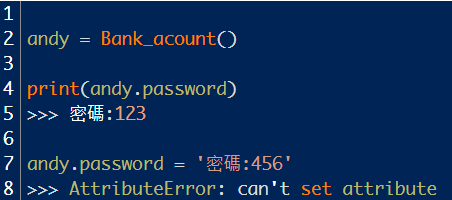
\includegraphics[width=0.7\linewidth]{1st property.png}
        \caption{Example Code}
        \label{2}
    \end{figure}
    \item There should be \textbf{getter}, \textbf{setter}, and \textbf{deleter}, if one would like to modify the data of \textbf{propertied} function.
\end{itemize}

If one touched C++ first like me, think about the difference of \textbf{private} and \textbf{public}.

\section{Dataset-X(self) and y(self)}
\begin{lstlisting}
@property
def X(self):
    return self._values

@property
def y(self):
    return self._label
\end{lstlisting}

Now we can see what \textbf{\_values[]} and \textbf{\_label} stand for.
 Recall that the function of ParticleNet would be labeling and identifying particles.
 Then we should recognize that \textbf{\_label} here represents the label of training data, and \textbf{\_values[]} would be the original data got from detector.
These shouldn't be able to be modified by the model during the training process, thus we use \textbf{@property} to protect them.

\section{Dataset-shuffle(self, seed=None)}
\begin{lstlisting}
def shuffle(self, seed=None):
    if seed is not None:
        np.random.seed(seed)
    shuffle_indices = np.arange(self.__len__())
    np.random.shuffle(shuffle_indices)
    for k in self._values:
        self._values[k] = self._values[k][shuffle._indices]
    self._label = self._label[shuffle_indices]
\end{lstlisting}

Line 2 to 3, we should make sure that \textbf{seed} isn't empty, if so we should set it to be Numpy random seed\footnote{\textbf{numpy.random.seed} function is used to initialize the random number generator with a seed. Seed ensures \textit{reproducibility} of random number generation, that is, using the same seed would result in the same sequence of random number.}.
\\\indent Line 4, it creates an array of indices from 0 to \textbf{self.\_\_len\_\_()}\footnote{Recall that \textbf{self.\_\_len\_\_()} is the function that measures the length of \textbf{\_label}.} using \textbf{np.arange}. 
This array represents the indices of the elements to be shuffled, that is, in this function, we shuffle the order of training data numbered by \textbf{\_label}.
\\\indent Line 5, shuffle the array effectively, arranging the values to indice indicated by \textbf{shuffle\_indices}.
\\\indent Line 6 to 7, going into for loop, it iterates the indices of \hyperref[sec:values]{\textbf{self.\_values}}. 
Recall that it is a dictionary whose value would be \textbf{stacked array}. Thus we go into the for loop and shuffle the content of \textbf{\_values} for each key according to \textbf{shuffle.\_indices}.
\\\indent Line 8, we shuffle \textbf{self.\_label} according to \textbf{shuffle.\_indices}.

\section{Transforming Data}
\begin{lstlisting}
train_dataset = Dataset('converted/train_file_0.awkd', data_format='channel_last')
val_dataset = Dataset('converted/val_file_0.awkd', data_format='channel_last')
\end{lstlisting}
First, we should know what \textbf{channel\_last} is. As implied by professor, it is the data format used in Numpy Array.
\section{channel\_last}\label{sec::channel}
This data format is a convention in operating image in deep learning, and there is an oppisite data format, that is, \textbf{channel\_first}.
The former more often appear in implementation.
We knew that typically, an image can be stored in three-dimension array.
Rows are for height, and columns are for width, and the remaining ones are for channel\footnote{Typically, there would be 3 channels, representing the colors, and one for blue, and one for red, and the other for yellow.}.  
\begin{itemize}
    \item \textbf{Channels last}: [rows][cols][channels]
    \item \textbf{Channels first}: [channels][rows][cols]
\end{itemize}

We should know the order of storing data because we're not manipulating image.
As \hyperref[sec::Appendices]{appendix} implies, \textbf{np.stack()} would preserve the data format.

\section{Importing model}
\begin{lstlisting}
import tensorflow as tf 
from tensorflow import keras
from tf_keras_model import get_particle_net, get_particle_lite
\end{lstlisting}
Note that the modulus package of ParticleNet model should be download locally and stored in the same folder in PC.

\section{Inputing the model}
\begin{lstlisting}
model_type = 'particle_net_lite'
#choose between 'particle_net' and 'particle_net_lite'
num_classes = train_dataset.y.shape[1]
input_shapes = {k:train_dataset[k].shape[1:] for k in train_dataset.X}
if 'lite' in model_type:
    model = get_particle_net_lite(num_classes, input_shapes)
else:
    model = get_particle_net(num_classes, input_shapes)
\end{lstlisting}

I think the most confusing code would be line 3 and 4. Here are some explanation. Line 3, note that in the model, our purpose is to label the unknown particles based on their properties.
 We simulated the desired process and then make the simulated data into training data, that is, we now assume there would only be limited kinds of particles identified by label, which is stored in \textbf{train\_dataset.y}.
 Thus, we classify the real data with same labels, that is line 3 doing, it equalizes the number of classes \textbf{num\_classes} with the number of labels in training data, or simulated data.
\\\indent
Line 4 is setting the size of the inputs, which is correspond to training dataset values.
Note that we ignore the first row of the training data, this is because of the convention in deep learning that this row would be preserved for \textbf{batch size}
\footnote{This is the number of independent data sheet that is thrown into each training in each epoch.}.

\section{Setting Training Parameters}
\begin{lstlisting}
#Training Parameters
batch_size = 1024 if 'lite' in model_type else 384
epochs = 30
\end{lstlisting}

\section{lr\_shedule}
\begin{lstlisting}
def lr_schedule(epoch):
    lr = 1e-3
    if epoch > 10:
        lr *= 0.1
    elif epoch > 20:
        lr *= 0.01
    logging.info('Learning rate: %f'%lr)
    return lr
\end{lstlisting}

This is the function that stands for \textbf{learning schedule} for different epoch. 
As one can see in the function, the learning rate would slow down when the training process is almost done.
The reason why the learning rate should slow down is due to several reasons. 
\begin{itemize}
    \item Convergence improvement: At the beginning of training, we set the high learning rate is because we want the model to converge faster.  As the optimization process progresses and the model approaches a minimum or a good solution, reducing the learning rate prevents overshooting and helps the optimizer to fine-tune the model more delicately. This can lead to improved convergence and better generalization.
    \item Escape local minima: At high learning rate, the model soon converges to a minimum, but this minimum may be mere local minimum, so we should slow down the learning rate that help us learn more around that minimum.
    \item Avoidance of Overshooting: High learning rates might cause the optimization process to overshoot the minimum, leading to oscillations or divergence. Gradually reducing the learning rate helps prevent such overshooting as the optimization process progresses.
\end{itemize}

\section{Model Information}
\begin{lstlisting}
model.compile(loss='categorical_crossentropy', optimizer = keras.optimizers.Adam(learning_rate = lr_schedule(0)), metrices = ['accuacy'])
metrics=['accuracy']
model.summary()
\end{lstlisting}
This piece of code setup the model using specified loss function, optimizer, and metrices.

\section{Prepare Model and Its Saving Directory}
\begin{lstlisting}
# Prepare model model saving directory.
import os
save_dir = 'model_checkpoints'
model_name = '%s_model.{epoch:03d}.h5' % model_type
if not os.path.isdir(save_dir):
    os.makedirs(save_dir)
filepath = os.path.join(save_dir, model_name)

# Prepare callbacks for model saving and for learning rate adjustment.
checkpoint = keras.callbacks.ModelCheckpoint(filepath=filepath, monitor='val_acc', verbose=1, save_best_only=True)
lr_scheduler = keras.callbacks.LearningRateScheduler(lr_schedule)
progress_bar = keras.callbacks.ProgbarLogger()
callbacks = [checkpoint, lr_scheduler, progress_bar]
\end{lstlisting}
This part would not be our focus.\\\\\\

\section{Training}
\begin{lstlisting}
train_dataset.shuffle()
model.fit(train_dataset.X, train_dataset.y, batch_size=batch_size, epochs=epochs, validation_data=(val_dataset.X, val_dataset.y), shuffle=True, callbacks=callbacks)
\end{lstlisting}

One can see that we first shuffle the training data to prevent overfitting, and then we fit the model.
\chapter{Appendices}\label{sec::Appendices}
Here is the code that one can check that for the same input data but stored in different data format
\footnote{That is, the code first assume the random data is stored in \textbf{channel\_first} and then convert the data format into \textbf{channel\_last}.}. 
We can see from the message in the terminal, the converted data format would be preserved.
\\\indent Here is the code:
\begin{lstlisting}
import numpy as np

# Create random data
data_shape = (3, 2, 1)  # Assuming 3 channels, 4 rows, and 5 columns
data_channel_first = np.random.rand(*data_shape)
data_channel_last = np.moveaxis(data_channel_first, 0, -1)  # Convert to channel_last

# Assume 'data_format' is set based on how the data is stored
data_format_channel_first = 'channel_first'
data_format_channel_last = 'channel_last'

class DataProcessor:
    def __init__(self, data_format):
        self.stack_axis = 1 if data_format == 'channel_first' else -1

    def process_data(self, data):
        # Some processing code here
        processed_data = np.stack([data, data, data], axis=self.stack_axis)
        return processed_data

# Create instances of DataProcessor for both formats
processor_channel_first = DataProcessor(data_format_channel_first)
processor_channel_last = DataProcessor(data_format_channel_last)

# Process data using both processors
result_channel_first = processor_channel_first.process_data(data_channel_first)
result_channel_last = processor_channel_last.process_data(data_channel_last)

# Print results
print("Check that they are really in channel first and channel last:\n")
print(data_channel_first.shape)
# print("\n")
print(data_channel_last.shape)
print("Initial data (channel_first):")
print(data_channel_first)
print("\nResult after processing (channel_first):")
print(result_channel_first)

print("\nInitial data (channel_last):")
print(data_channel_last)
print("\nResult after processing (channel_last):")
print(result_channel_last)

print("\nThe difference can be seen by checking their shape:")
print(result_channel_first.shape)
print("\n")
print(result_channel_last.shape)
\end{lstlisting}
\end{document}